As we already explained in the section xx \fxnote{add here the ref for section where transcription process is explained}, the main objective of this work is to predict the \Gls{tr} of a cell, given a map of the proteins inside the cell. For this we use \textit{Multiplexed Protein Maps}.

Accordingly with \cite{Guteaar7042}, \textit{Multiplexed Protein Maps} (in case of the paper, 40-plex) are protein readouts from biological samples obtained by \Gls{4i}. This method simultaneously captures different properties of the cell, like its shape, cycle state, detailed morphology of organelles, nuclear subcompartments, etc. It also captures highly multiplexed subcellular protein maps, which can be used to identify functionally relevant single-cell states, like \Gls{tr}.

Therefore, how to get the multiplexed protein map of a single cell? First, lets explain briefly how does \gls{4i} work.

Roughly speaking, given a population of cultured cells (human tissue), a specific protein inside the cells is stained with a fluorescent antibody. Then, the tissue is exposed to high-energy light and photographed. After that, the fluorescent antibody is removed by an elution process from the tissue, to start the process again but with another fluorescent antibody. This process is repeated several times to photograph the concentration and distribution of around 40 different proteins inside the cell. Finally, by means of computer vision algorithms\fxnote{should I add the reference to the papers where this is explained?? ref 22-24 and 30}, each cell in the photographed tissue is identified, segmented (Nucleus and Cytoplasm) and saved separately. It is also important to mention that for this process, the tissue is located in a gridded plate, where each grid (called \hl{Well}) contains several cells. The \gls{4i} process can be observed in figure \cref{fig:4i}

\fxnote{The last paragraph explain only in general the whole process to get a single cell image. However, should I add also the explanation of the \gls{4i} protocol? \ie the process of 21 cycles of staining-elution, image composition, etc.?}

\begin{figure}[htb]
  \centering
  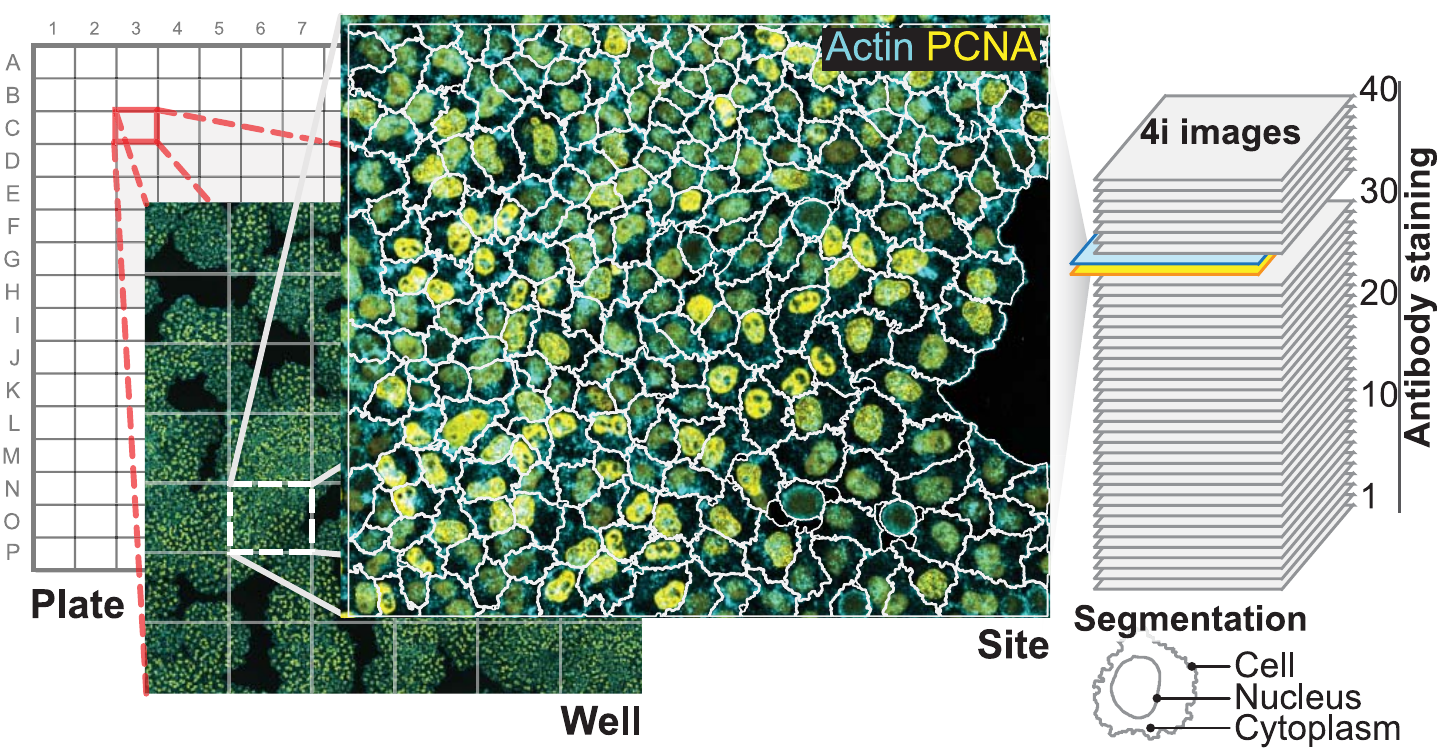
\includegraphics[width=100mm]{./Sections/Images/plate-well.png}
  \caption{\Acrlong{4i} process. Image source \cite{Guteaar7042}.}
  \label{fig:4i}
\end{figure}
